\documentclass[12pt]{article}

\usepackage{geometry}
\geometry{a4paper}
\geometry{margin=2.5cm,top=2cm,bottom=2cm}

\usepackage{fancyhdr}
\pagestyle{fancy}
\renewcommand{\headrulewidth}{0.4pt}
\renewcommand{\footrulewidth}{0.4pt}
\renewcommand{\sectionmark}[1]{ \markright{#1}{} }
\lhead{Cyril NOVEL (cbn13)}\chead{}\rhead{\textit{ \nouppercase{\rightmark}}}
\lfoot{}\cfoot{\thepage\ of \pageref{LastPage}}\rfoot{}

\setlength{\headheight}{15pt}


\usepackage[english]{babel}
\usepackage[utf8]{inputenc}
\usepackage{amsmath}
\usepackage{graphicx}
\usepackage{algpseudocode}
\usepackage{algorithm}
\usepackage{amsthm}
\usepackage{amssymb}
\usepackage{mathtools}
\usepackage{commath}
\usepackage{stmaryrd}

\title{Surface reconstruction\\
\large{CO512 ISO Report}}

\author{Cyril NOVEL}

\date{\today}

\begin{document}
\maketitle
\newpage

\tableofcontents

\newpage

\addcontentsline{toc}{section}{Introduction}
\section*{Introduction}
In the last decades, numerous devices have been developped in order to capture and digitize our world. Among them, 3D scanners aim at capturing the geometry of the objects surounding us. Statues, monuments but also industrial parts, landscapes : all these can be digitized into a 3D point cloud. But a 3D point cloud isn't enough for a correct visualization by human beings. Thus the reconstruction of the surface is needed to obtain a more comprehensible object.

Because of the numerous fields it covers -- cultural, industrial, medical -- Surface reconstruction is a widely studied subject in Computer Science. In this report, we will present the three main categories of algorithms used to perform surface reconstruction. For each category we will describe two or more precise algorithms.

\newpage

\section{Delaunay-based algorithms}
Delaunay-based algorithms are based on the Delaunay triangulation of a point cloud and the Voronoi diagram of a point cloud. In 2D, a Delaunay triangulation of a set of points $P$ is a triangulation such that no point in $P$ is inside the circumcircle of any triangle of the triangulation. We can generalize Delaunay triangulation in a $n$-dimension space, using simplex. For surface reconstruction, $n = 3$ so that the property becomes : a Delaunay triangulation of a set of points $P$ such that no point in $P$ is inside the circumspeher of any tetrahedron of the triangulation.

A Voronoi diagram is a way to divide the space. Given a set of points $\{p_i\}$,  for each point there will be a corresponding region $R_i = \{x | dist(p_i,x) < dist(p_j,x) ; i \ne j\}$. The regions are called Voronoi cells.

The Voronoi diagram is the dual of the Delaunay triangulation.

\subsection{General idea}
The Delaunay-based algorithm can be divided into two main steps. First, it computes a geometric triangulation of the finite set of points via the Delaunay triangulation or the Voronoi diagram. Then, it extracts a collection of facets chosen so that they are close to the actual surface.

The advantage of Delaunay-based algorithms is that the triangulation created is more robust than other approaches. Delaunay triangulation comes with a variety of theoretical guarantees. However, the Delaunay triangulation is very expensive to compute, thus these algorithms are very expensive for large point clouds.

We describe two different Delaunay based algorithms : the Power Crust algorithm and the Cocone algorithm.

\subsection{Power crust algorithm}
\label{subsec:pca}
The Powercrust algorithm -- described in \cite{Powercrust}-- compute an approximate medial axis of the 3D point cloud $S$ using the Voronoi diagram. We then take a subset $V$ of the Voronoi vertices, called the poles. The poles lie near the medial axis. Each pole has an associated ball, called the polar ball. The polar balls approximate maximal balls contained in the interior or exterior of the 3D shape. The radii of the polar balls are the weights of the poles. The inverse transform is then approximate using the power diagram using the set of weighted poles.

The Power Crust algorithm can be summarize in 6 steps :
\begin{enumerate}
\item Compute the Voronoi diagram of the sample points $S$.
\item For each sample point, compute its poles.
\item Compute the power diagram of the poles.
\item Label each pole either inside or outside.
\item Output the power diagram faces separating the cells of inside and outside poles as the power crust.
\item Output the regular triangulation faces connecting inside poles as the power shape.
\end{enumerate}

The Power crust algorithm uses the notion of the \textit{Medial Axis Transform}. Let $F$ be the boundary of the 3D object. To avoid infinity edges and/or points, we assume that $F$ is contained in a bounded open region $Q$ -- for example a 3D box containing $F$. $F$ divides $Q$ into interior and exterior solids. Let $B_{c,r}$ be a ball of center $c$ and radius $r$. $B$ is empty if the interior of $B$ contains no point of $F$. A medial ball is a maximal empty ball, meaning that no other empty ball can completely contain it. The center of this medial ball is either a center of curvature of $F$ or a point with more than one closest point on $F$.

The \textit{Medial Axis Transform} of $F$ is the set of medial balls of F. The centers of the medial balls form the medial axis of $F$. The medial axis includes a part inside of $F$ and a part outside of $F$. The medial axis of a three-dimensional object is generally a two-dimensional surface.

Assuming a dense sampling, the Voronoi cell of every point of the data set is long, skinny and \textit{perpendicular} to the surface. It happens because in directions tangent to the surface the Voronoi cell is limited by the very close neighbors. So the Voronoi cell extends perpendicularly away from the surface and cannot extend farther than the medial axis. There it is not the closest point anymore -- due to the nature of the medial axis. Thus, the Voronoi vertices at the two ends of the long, skinny Voronoi cell should lie near the median axis. This motivates the selection of poles as an approximation of the median axis.

In pratice, the selection of the poles is done as follow : compute the Voronoi diagram of $S$, with a surrounding box of 8 vertices in order to avoid infinite edges. For each point $s \in S$, find the farthest vertex of the corresponding Voronoi cell, $p_1$. $p_1$ is the first pole of $s$. Then find the farthest vertex $p_2$ of the corresponding cell, such that $p_2.p_1 < 0$. $p_2$ is the second pole of $s$.

The inverse transform uses a \textit{power diagram}. A finite set of balls can be related to power diagrams, which are a kind of Voronoi diagrams, using the distance function :
$$d_{pow}(x, B_{c,r}) = d^2(c,x) - r^2$$
with $d$ the usual distance function in an euclidean space  $B_{c,r}$ the ball of center $c$ and radius $r$. Note that if $x$ is inside $B_{c,r}$, $d_{pow}$ is negative. We use $d_{pow}$ to define a Voronoi diagram, called the \textit{power diagram}.

Considering the power diagram of the polar balls, the \textit{power crust} is the boundary between the power diagrams cells belonging to inner poles and power diagramms cells belonging to outer poles. A facet of the power crust separates cells corresponding to an inner and an outer pole. With a dense sampling, the two polar balls should intersect only slightly, since the inner ball is mostly inside the object and the outer ball outside. The power crust actually interpolates the points of the original point cloud.

The previous paragraph stresses the fact that we need to label the poles as inner poles or outer poles. We define a graph such that two cells are connected in the graph if they share a two-dimensional face. Moreover, two faces are connected of they belong to the poles generated by the same point $s$. When $S$ is well-sampled, two properties can be extracted. The first is that an inner polar ball and an outer polar ball can only intersect shallowly. The second is that every sample as one unique inner pole and one unique outer pole. 

The first way to label the cells -- and therefore the poles -- is via a naive algorithm. It begins by labeling poles adjacent to the points of the bounding box as outer poles and propagates labels as follows. For any pole $p$ labeled outer, if it has an unlabeled neighbor $q$ such that the polar balls of $p$ and $q$ intersect deeply, we label $q$ as outer. Else, we label it as inner. Similarly for the inner poles: deeply intersecting polar balls get labeled as inner, else get labeled outer. The deepness of the intersection is calculated by the angle formed by the 2 tangent planes at the intersetion of the two polar balls.

Unfortunately, the sampling assumption is not true everywhere. If an error is made in the previous labelling algorithm, it propagates and leads to a wrong surface. A solution is to keep track of the belief that an unlabeled ball is inner or outer, based on the labels already assigned. Each ball keeps track of two values between 0 and 1. One value is the belief that the ball is in, the other the belief that the ball is out. If $belief(in) = 1$, we are certain that the ball is an inner ball. If $belief(in) = 0$, the state of the ball is unknown. We initialize all poles close to the bounding box to $belief(out) = 1$ and for all the other balls', $belief(in) = belief(out) = 0$.
All the remaining unlabeled poles are put in a priority queue. The priority is determined by the $belief(in)$ and $belief(out)$ values. If one of these two values is zero, we use the other for the priority queue. If both are non-zero, the pole is \textit{confused} and is assigned priority $|in - out| - 1$, which is between 0 and -1.

Then repeatedly, we remove the top element of the queue and label it inner or outer, depending on the biggest value. We then computes the new belief values for the remaining poles. If $p$ and $q$ are the two poles of a sample point $s$, $\beta$ denotes the angle between $p,s$ and $q,s$. We have $\pi/2 < \beta < \pi$. The bigger $\beta$ is, the more likely it is that $q$ shoud get opposite label from $p$. So we use $0 \le -cos\beta \le 1$ as the weight of the connection between $p$ and $q$. We note $tmp(p)$ the maximum value of $belief(in)(p)$ and $belief(out)(p)$. If $p$ is labeled as inner, then $belief(out)(q) = max(tmp(p)*-cos\beta, belief(out)(q))$.

We know that two balls with different lables intersect shallowly. So the deeper the intersection, the more likely the two balls will have the same label. So we set the weight to be $0 \le -cos\alpha \le 1$. So if $p$ is labeled as inner, then $belief(in)(q) = max(tmp(p)*-cos\alpha, belief(in)(q))$.

We have the two rules for updating the priority queue. We just have to loop until every pole is labeled, and then extract the power crust.

For a better reconstruction, it is possible to omit certain poles. In the case of a noisy data set, some Voronoi cells are not well shaped, as we can see in figure~\ref{noisePC}.
\begin{figure}[h]
  \centering
  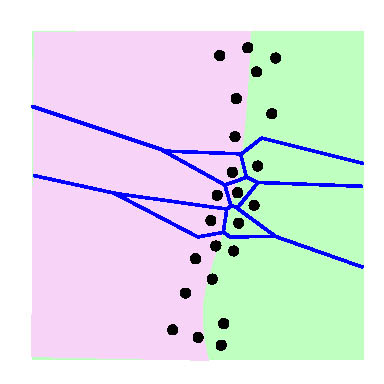
\includegraphics[scale=0.3]{noise.jpg}
  \caption{\label{noisePC} Oddly shaped Voronoi cells due to noise in the data.}
\end{figure}

Some cells are round, others don't have perpendicular borders. It is possible to discard this cells and so the poles in order to build a better MAT. 

Oddly shaped cells appears also for sharp egdes. If all the cells are kept, the reconstruction is too smooth and we loose the information about the sharpness of the surface. Discarding some cells allows a better reconstruction, as shown by figure~\ref{sharpPC}.

\begin{figure}[h]
  \centering
  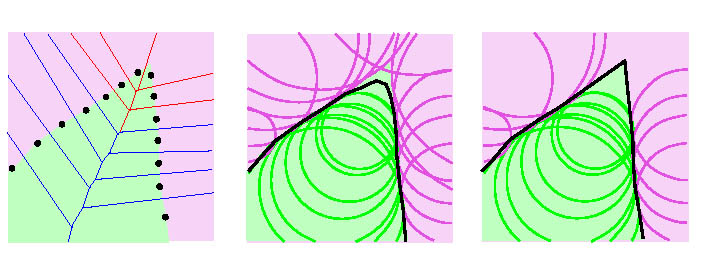
\includegraphics[scale=0.3]{sharpPC.jpg}
  \caption{\label{sharpPC} Influence of the cells on a sharp feature.}
\end{figure}

\subsection{Cocone algorithm}
The Cocone algorithm is also a Delaunay-based algorithm, described in \cite{Cocone}. The idea here is to find the restricted Delaunay Triangulation according to the surface of the 3D model. Edelsbrunner and Shah showed that the underlying space of this triangulation is homeomorphic to $S$ under certain conditions. To find the restricted Delaunay Triangulation $DT_S$, we consider the restricted Voronoi diagram $V_S$ with restricted Voronoi cells $V_{s,S} = V_s\cap S$. The dual of this restricted Voronoi diagram is $DT_S$. More precisely, the edge $pq \subset DT_S$ if and only if $V_{p,S}\cap V_{q,S} \ne \emptyset$. A triangle $pqr \subset DT_S$ if and only if $V_{p,S}\cap V_{q,S}\cap V_{r,S} \ne \emptyset$.

The homeomorphic condition is called \emph{closed ball properties} and states that each $V_{s,S}$ is a topological 2-ball, each non-empty intersection $V_{p,S}\cap V_{q,S}$ is a topological 1-ball and each non-empty intersection $V_{p,S}\cap V_{q,S}\cap V_{r,S}$ is a point. Under this condition, $DT_S$ is a piecewise linear manifold homeomorphic to $S$.

We introduce also the \emph{local feature size}, $f(s)$. $f(s)$ -- $s \in S$ -- is the least distance between $s$ and the medial axis of $S$. $f$ is 1-Lipschitz, meaning $\abs{f(p) - f(q)}\le\abs{p - q}$.

The \emph{cocone} algorithm selects a set of candidates triangles $T$ satisfying three conditions:
\begin{enumerate}
\item $DT_S \subset T$.
\item The circumcircle of each triangle $t \in T$ is small.
\item The normal to each triangle $t \in T$ makes a small angle $c\epsilon$ with the surface normal at the vertex $s$, where $s$ is the vertex with the largest angle in $t$ and $c$ is a constant independant of $\epsilon$.
\end{enumerate}

Let $S$ be the actual surface of the 3D model, $D$ the data set and $s \in D$ a point of the data set. We start by comptuing the Voronoi diagram $V$ of $D$. For every point $s \in D$, we call $V_s$ the associated Voronoi cell. The normal to $S$ at a point $s$ is estimated using the farthest pole of $V_s$, as introduced in the subsection~\ref{subsec:pca}. The estimated normal is the line going through $s$ and that pole. We then find the complementary cone -- \emph{cocone} -- of $V_s$. The \emph{cocone} is defined as the complement of the double cone of apex $s$ making an angle of $\frac{\pi}{2}-\theta$ with the estimated normal at $s$. In practice, $\theta\le\frac{\pi}{8}$. In figure~\ref{coc}, the cocone is the space between the two grey zones.

\begin{figure}[h]
  \centering
  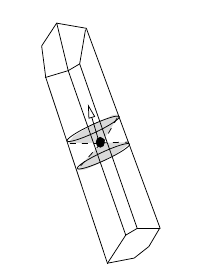
\includegraphics[scale=0.3]{Cocone.png}
  \caption{\label{coc} Cocone of a Voronoi cell}
\end{figure}

We then select the edges of $V$ that intersect the cocone of their three adjacent samples. The dual triangles of these edges form the candidate set of triangles $T$. Under the assumption $\theta\le\frac{\pi}{8}$, $T$ satisfies the three conditions stated before.

The next step is to remove all triangles incident to sharp edges. An edge is sharp if the angle between two consecutive triangles around this edge is superior to $\frac{3\pi}{2}$. An edge with a single incident triangle is also sharp.

Once this set is performed, the remaining triangles set is the surface of the 3D object. However, it has been shown that in pratice, Cocone algorithm produce a lot of holes in the surface. \cite{Tightcocone} introduces a Water-tight cocone algorithm which produces a water-tight surface of the 3D model.

%% ADD HERE WATER TIGHT COCONE %%

\newpage

\section{Region-growing algorithms}
\subsection{General idea}
A classic region-growing algorithm begins by initiating a triangle as an initial region and then iterates to link new triangles on the region's boundaries. This type of algorithm is very fast. Most of the time, each point of the point cloud is considered only once for the triangulation. The disadvantage is that the reconstruction relies heavily on parameters chosen by the user and on the sampling of the point cloud. Moreover this method can create small holes in the surface when poor data  exists -- due to noise for example. 

We describe two different region-growing algorithms : the Ball Point algorithm and the Fast Reconstruction algorithm of the Point Cloud Library.

\subsection{Ball Point algorithm}
The idea of the BPA is very simple : three points form a triangle if a ball of radius $\rho$ touches them without containing any other points. Starting with a seed triangle, the sphere pivots around an edge of the triangle until it touches another point. It then formed a new triangle. We loop this process until all reachable edges have been considered. We give an illustration of the processus in 2D in figure~\ref{bpa2D}.

\begin{figure}[h]
  \centering
  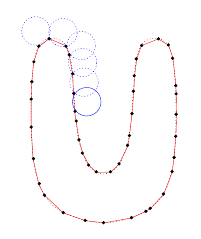
\includegraphics[scale=0.5]{BPA.png}
  \caption{\label{bpa2D} The BPA in 2D.}
\end{figure}


Let $M$ be the surface of the 3D object and $S$ be the sampling points of $M$. For every point $s \in S$, we have the geometric position and the normal orientation. We make a sampling assumption: $S$ is dense enough so that no ball with radius $\rho$ can go through the surface without touching sample points.

% HERE SAMPLING ASSUMPTIONS

The BPA works by finding a seed triangle and use an advancing front to track which points have been visited and which are in the current boundary. The front $F$ is a collection of linked lists of edges. It is initialized by a single loop containing the three edges defined by the seed triangle. Each edge is represented by its two end points, the opposite vertex and the center of the ball that touches all three points. We classify the edge as \textit{active} or \textit{boundary}. An \textit{active} edge will be used for pivoting. If the pivoting is impossible, then we classify it as \textit{boundary}. This information about the states of the edges allows a simpler and clearer algorithm for the pivoting of the ball. We do not use a single linked list because when the ball pivots around an edge, it can reach a new data point or a previously seen data point. Depending on this, the front changes topology. Algorithm~\ref{alg:bpa} shows the pseudocode for the Ball Pivoting Algorithm.

\begin{algorithm}
\caption{Ball Pivoting Algorithm}
\label{alg:bpa}
\begin{algorithmic}[5]
\While{$true$}
  \While{$e_{i,j} = get\_active\_edge(F)$}
    \If{$s_k = ball\_pivot(e_{i,j}) \&\& (not\_used(s_k) \| on\_front(s_k))$}
      \State $output\_triangle(s_i, s_k, s_j)$
      \State $join(e_{i,j}, s_k, F)$
      \If{$e_{k,i} \in F$}
        \State $glue(e_{i,k}, e_{k,i}, F)$
      \EndIf
      \If{$e_{j,k} \in F$}
        \State $glue(e_{k,j}, e_{j,k}, F)$
      \EndIf
    \Else
      \State $mark\_as\_boundary(e_{i,j})$
    \EndIf
  \EndWhile

  \If{$(s_i, s_j, s_k) = find_seed_triangle()$}
    \State $output\_triangle(s_i, s_j, s_k)$
    \State $insert\_edge(e_{i,j}, F)$
    \State $insert\_edge(e_{j,k}, F)$
    \State $insert\_edge(e_{k,i}, F)$
  \Else
    \State $return$
  \EndIf
\EndWhile
\end{algorithmic}
\end{algorithm} 

%\newpage 
Two functions -- $ball\_pivot$ and $find\_seed\_triangle$ -- need an efficient way to retrieve the neighbourhood of a point. A simple solution is using a grid of small cubes, called voxels. The voxel's side is $\delta = 2\rho$. We store the data points in a list for each voxels. Given a point $s$, we can find the voxel $v$ it lies in by divided its coordinates by $\delta$. In order to look at every point that lies at a distance $\rho$ of $s$, we need to look at all the neighbours of $v$. Hence a total of 27 voxels to consider.

The selection of a seed is necessary for the initialisation of the pivoting. A seed triangle is a triangle such that a $\rho$ ball with its center in the outward space touches the three points of the seed triangle and contains no other data points. A way to find a seed triangle is :
\begin{itemize}
\item Pick any point $s$ not yet used by the triangulation;
\item Consider all pairs of point $s_1$, $s_2$ in the 27 voxels around $s$;
\item Build triangle $s_1$,$s_2$,$s$;
\item Orient the triangle normal thanks to the point normals;
\item Test that a $\rho$ ball with its center in the outward space touches the three points of the seed triangle and contains no other data points;
\item Stop when a valid seed triangle has been found.
\end{itemize}

The second step can be refined by selecting $s_1$ and $s_2$ such that they are at a distance less than $\rho$ from $s$. We can limit ourselves to one point per voxel as candidate vertex for the seed triangle. Also, for a given voxel we can average the normal of all the points, which approximates the surface in that region. Then we consider first points $s$ such that the projection of their normals on the average normal is largely positive.

The pivoting operation starts with a triangle $t =(s_i, s_j, s_0)$ and a $\rho$ ball that touches its three vertices. Let $e_{i,j}$ be the pivoting edge. The ball initially contains no other points than the points of $t$. Let $c_{i,j,0}$ be the center of the initial ball. When we are pivoting the ball around $e_{i,j}$, the center $c_{i,j,0}$ describes a circle which lies in the plan perpendicular to $e_{i,j}$ and passing by the midpoint $m = 1/2 * (s_i + s_j)$. The center of the circular trajectory is $m$ and the radius is $\| c_{i,j,0} - m \|$. If during the pivoting we hit a new point $s_k$, the triangle $(s_i, s_k, s_j)$ is a new valid triangle and the ball contains no other points, so it is valid for the next pivoting step. If we don't hit a new point, then $e_{i,j}$ is marked as boundary.
In pratice, we consider all points in the 27 voxels around $m$. For each point $s_x$, we compute -- if possible -- the center $c_x$ of the $\rho$ ball that touches $s_x$, $s_i$ and $s_j$. $c_x$ lies on the circular trajectory describes previously. Among all the $c_x$ points, we select the one that comes first along this trajectory -- via a simple angle computation. We now have the new triangle and the new center of the ball.

Once the new triangle is find, we have to update the front information. The \textit{join} operation is used when the ball pivot around $e_{i,j}$ and touches a \textit{not\_used} vertex $s_k$. In that case, we output the triangle and locally modify the front by removing $e_{i,j}$ and adding $e_{i,k}$ and $e_{k,j}$. If $s_k$ is already part of the mesh, two possibilities arise:
\begin{enumerate}
\item $s_k$ doesn't belong to the front. We don't generate the triangle since it would produce a non manifold mesh. Here $e_{i,j}$ is marked as boundary edge.
\item $s_k$ belongs to the front. We check edge orientation to orient correctly the ouput triangle, then we apply the \textit{join} operation. This operation can create one or two pairs of coincident edges.
\end{enumerate}

The coincident edges are removed by the \textit{glue} operation. Coincident egdes always have opposite orientation. For example, when edge $e_{i,k}$ is added by \textit{join}, if $e_{k,i}$ is on the front, \textit{glue} will remove the two edges. Two cases arise:
\begin{enumerate}
\item $e_{i,k}$ and $e_{k,i}$ are in the same linked list. We just have to removed them, since they are consecutive in the linked list.
\item $e_{i,k}$ and $e_{k,i}$ are in different linked lists, respectively $l_1$ and $l_2$. We remove $e_{i,k}$ from $l_1$ and called $l_{1,start}$ the first part of $l_1$ and $l_{1,end}$ the last part of $l_1$. We do the same thing with $l_2$. Then $l_1 = l_{1,start}+l_{2,end}$ and $l_2 = l_{2,start}+l_{1,end}$.

The join and glue operations are illustrated in figure~\ref{joinglue}.

\begin{figure}[h]
  \centering
  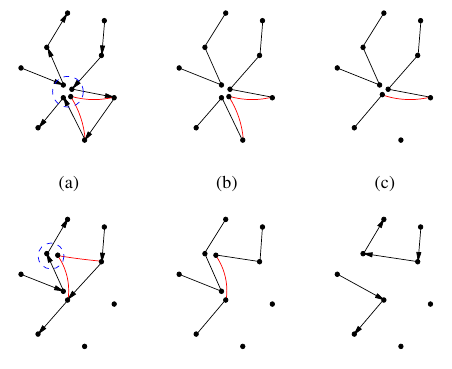
\includegraphics[scale=0.5]{joinglue.png}
  \caption{\label{joinglue} Illustration of join and glue operations. (a) A new triangle is added to the existing front. The four vertices inside the circle all represent a single data point. (b) A join operation removes an edge and creates two new front edges, coincident with existing ones. (c) A glue operation removes one edge. (d) A second glue operation removes the other edge. A new triangle is to be added. (e) Only one of the edges created by this join is coincident with an existing edge. (f) One glue removes the duplicate pair.
}
\end{figure}

%% FINISH PARAGRAPH

\end{enumerate}


\subsection{Fast Reconstruction algorithm (PCL)}
The Point Cloud Library is an open-source library for processing point clouds. It provides a greedy algorithm for reconstructing a surface from an unorganized point cloud as fast as possible, described in \cite{PCL1}. The idea is simple: for each point $s$, project its neighbourhood on the average plane, add edges according to visibility and go back to the 3D space. The algorithm is largely inspired by \cite{PCL2}, which we are going to describe.

This algorithm requires 2 parameters : $\mu > 1$ and $\alpha$. $\mu$ quantifies the idea of locally uniform sampling. $\alpha$ gives an upper bound on the angle between consecutive neighbors of a point on a boundary surface. $\alpha$ is a large angle, set at 120 degrees. The data points are categorized as \textit{free}, \textit{fringe}, \textit{boundary} or\textit{completed}. \textit{Free} points have no incident triangles. Points on the current boundary are labeled as \textit{fringe} or \textit{boundary}: a \textit{fringe} point has already been processed but have some missing triangles around it due to $\alpha$; a \textit{boundary} point has not yet been processed. The algorithm keep two properties true during its execution :
\begin{itemize}
\item No \textit{free}, \textit{fringe} or \textit{boundary} point can be in the interior of a triangle.
\item At the end of each iteration, the point processed is either labeled \textit{completed} or \textit{boundary}.
\end{itemize}

The neighbourhood of $s$ is defined by all the points that are in the sphere centered at $s$ and of radius $\mu m$ where $m$ is the distance between $s$ and its closest neighbour. This sphere is called sphere of influence around $s$. The selected points are called the candidate points and the set is noted $C_s$. Note that a point $p$ can be in the sphere of influence of $s$ and $s$ doesn't lie in the sphere of influence of $p$. However this asymmetry doesn't have an impact on the toplogy of the reconstructed mesh. Different techniques can be used to find the points in the sphere of influence. We can use an octree structure, a voxel grid or a kd-tree.

The triangulation around $s$ is made on the projection plane $P_s$. The choice of $P_r$ is crucial for the robustness of the algorithm. The best plane would be the tangent plane of the actual surface, but it is very expensive to compute -- since we are looking for the surface. A fast approach can be averaging the normals of the existing triangles incident to $s$. Another solution is to compute the least square plane with the covariance matrix of the points in the sphere. Once the plane is found, we project the points in $C_s$ on the plane and called the resulting set of points $C^p_s$.

The next step is to order the points in $C^p_s$ around $s$. We define the coordinate system of $P_s$ with $s$ as the origin. Each point is characterized by the angle $\theta$ between the $x$ axis and the vector from $s$ to the point. Then $C^p_s$ is partitioned by the quadrants in which they lie. In each quadrant, we sort the points based on $sin^2(x)$. These ordered sets are merged and thus we have the angle ordering around $s$.

Among the points in $C^p_s$, some points are not visible from $s$. We have to remove them from the set before performing the triangulation step. We define a \textit{boundary edge} as any edge with only one triangle incident on it. The point of a \textit{boundary edge} therefore have to be labeled as \textit{fringe} or \textit{boundary}. \textit{Internal edges} are edges connecting a \textit{completed} point to any other points. The \textit{boundary} edges are also projected on $P_s$. If the line of sight from $s$ to a point in $C^p_s$ is obstructed by an edge, then the point is occluded and removed from $C^p_r$. All the points between consecutive \textit{boundary edges} of $s$ are removed as the can't be seen from $s$. Then we can remove \textit{fringe} or \textit{boundary} that have $s$ in their invisible region. Once this is done, we test the remaining points for occlusion. The naive approach of considering all the edges for occlusion is very expensive. The following theorem limits the search to few edges:
\newtheorem{mydef}{Theorem}
\begin{mydef}
Only the \emph{boundary edges} of the points in $C_s$ can be possible occluding edges between $s$ and $C^p_s$.
\end{mydef}

The remaining points are ordered and stored in $C^f_s$. Then we perform the triangulation step. The points in $C^f_s$ are connected to $s$. If the angle between two consecutive points is less than $\alpha$, the two points are connected with a \emph{boundary edge}. If an edge already exists, then we label it as an \emph{internal edge}. If the angle is greater than $\alpha$, then the two points are not connected to each others. We label the edges starting from $s$ accordingly to the triangles formed. If $s$ is surrounded by triangles, $s$ is labeled as \emph{completed}. Else $s$ is labeled as \emph{boundary}. All the \emph{free} points in $C^f_s$ are labeled as \emph{fringe} points and are append to the queue of points to process. An illustration of the triangulation step is given in figure~\ref{proj}.

\begin{figure}[h]
  \centering
  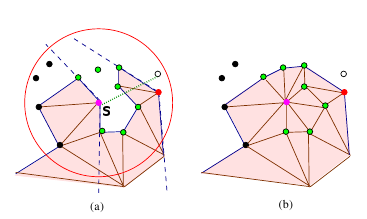
\includegraphics[scale=0.5]{proj.png}
  \caption{\label{proj} (a) is an illustration of the visibility pruning around $s$. The black points are behind $s$ and can not be seen. The visibility for the red point shows that $s$ is invisible to the red point, thus the red point is invisible to $s$. The white point is occluded by boundary edges. (b) Completed mesh at $s$.
}
\end{figure}

%% FINISH PARAGRAPH

\newpage

\section{Implicit surface algorithms}
\subsection{General idea}
In an implicit surface algorithm, an indicator function $f$ is computed from the sample points. $f:\mathbb{R}^3 \to \mathbb{R}$ can be positive inside the 3D model and negative outside the 3D model. Or $f$ can be equal to $0$ outside the model and equal to $1$ inside the model. Given $f$, we extract the right isosurface that fits the actual surface of the 3D model.

There is a major difference between Implicit surface algorithms and Region-growing or Delaunay-based algorithms. Region-growing and Delaunay based methods interpolate sample points, mean that the reconstructed surface lies on the sample points. The implicit surface approach approximates sample points and can lack accuracy. But one advantage is that implicit surface methods are ideal in the case of highly noised data.

We describe four different implicit surface algorithms : the Poisson algorithm, the Radial Basis Function algorithm, the Level Set algorithm and the Marching Cubes algorithm.


\subsection{Poisson algorithm}
In the Poisson algorithm, we compute an \emph{indicator function} $\chi$, defined as 1 at points inside the 3D object, 0 otherwise. We obtain the reconstructed surface by extracting the right isosurface. The main idea is that there is a relationship between the sampled oriented points and the indicator function of the model. The gradient of $\chi$ is  a vector field that is zero almost everywhere, since $\chi$ is constant almost everywhere. At points near the surface however, the gradient of $\chi$ is equal to the inward surface normals. So the oriented samples can be viewed as samples of the gradient of $\chi$.

The goal is to find the function $\chi$ whose gradient best approximates the vector field $\vec{V}$ defined by the given oriented points. So we have to solve $min_\chi\|\nabla\chi - \vec{V}\|$. By applying the divergence operator, this problem becomes a Poisson problem: find $\chi$ whose Laplacian -- divergence of gradient -- equals the divergence of $\vec{V}$:
$$\Delta\chi = div(\vec{V})$$

Let $S$ be the input data, with $s \in S$ a sample consisting of $s.p$ the position and $s.\vec{N}$ the inward facing normal. We assume $s$ is lying on or near the surface $\partial M$ of an unknow model $M$.

Because $\chi$ is a piecewise constant function, its explicit gradient field would result in a vector field with unbounded values at the surface boundary. To avoid this problem, $\chi$ is convolve with a smoothing filter and we consider the gradient field of the smoothing function.

\newtheorem{lemma}{Lemma}
\begin{lemma}
Given $M$ and its boundary $\partial M$, let $\chi_M$ be the indicator function of $M$, $\vec{N}_{\partial M}(p)$ be the inward facing normal at $p \in \partial M$, $\tilde{F}(q)$ be a smoothing filter and $\tilde{F}_p(q) = \tilde{F}(q-p)$ its translation to the point $p$. The gradient of the smmoothed indicator function is equal to the vector field obtained by smoothing the surface normal field:
$$\nabla(\chi_M * \tilde{F})(q) = \int_{\partial M} \tilde{F}_p(q) \vec{N}_{\partial M}(p) dp$$
\end{lemma}

The problem is that we don't know what the surface $\partial M$ is and thus we can't perform the integration. We approximate the gradient field with a discrete summation on the sample points. We use them to sample $\partial M$ into distinct patches $P_s \subset \partial M$ and approximate the integral:
$$\nabla(\chi_M * \tilde{F})(q) \approx \sum_{s \in S} \\|P_s\\| \tilde{F}_{s.p}(q) s.\vec{N} \equiv \vec{V}(q)$$

The choice of the smoothing filter is in pratice important. On the one hand, it should be sufficiently narrow so that the data is not oversmooth. And on the other hand it should be wide enough so that the integral over $P_s$ is well approximated by the value at $s.p$ times the patch area. A good choice of filter that balances these two requirements is a Gaussian filter whose variance is on the order of the sampling resolution.

For the implementation, we must discretize the problem. The idea here is to use a set of function to represent $\chi$ as a combination of those functions. A straightforward approach is to discretize the space with a regular 3D grid. But this uniform structure becomes impractical for fine detail reconstruction. Moreover, some areas are finely details whereas there is no points in them.

We only need an accurate representation of the implicit function near the surface. This motivates the use of an adaptative octree to represent the implicit function and to solve the Poisson system. An octree is a tree data structure in which each node has exactly eight children. In 3D space, each node is a cube, and its children are smaller cubes, dividing the node into 8 equal cubes. We use the positions of the sample points to define the octree $O$ and associate a function $F_n$ to every node $n \in O$. The following conditions have to be satisfied:
\begin{enumerate}
\item $\vec{V}$ can be precisely and efficiently represented as the linear sum of the $F_n$.
\item The matrix representation of the Poisson equation, expressed in terms of the $F_n$ can be solved efficiently.
\item A representation of the indicator function as the sum of the $F_n$ can be precisely and efficiently evaluated near the surface model.
\end{enumerate}

Given $S$ and a maximum tree depth $D$, We define the octree $O$ to be the minimal octree such that every point sample fall into a leaf node at depth $D$. We then define a set of functions obtain as the span of a fixed, unit-integral base function $F: \mathbb{R}^3 \to \mathbb{R}$. For every node $n$, we define $F_n$:
$$F_n(q) = F(\frac{q - n.c}{n.w})\frac{1}{o.w^3}$$
where $n.c$ is the center of the node and $n.w$ is the width of the node.

The space of functions $\{F_n\}$ has a multiresolution structure: deeper nodes are associated with higher frequency functions. Due to the octree representation, the function representation becomes more precise as we are closer to the surface.

%% SELECTION OF THE BASE FUNCTION %%

To obtain a better precision, we use trilinear interpolation to distribute the sample accross the eight nearest node. We define the approximate gradient field of the indicator function as:
$$\vec{V}(q) \equiv \sum_{s \in S} \sum_{n \in Ngbr_D(s)} \alpha_{n,s}F_n(q)s.\vec{N}$$
where $Ngbr_D(s)$ are the 8 depth-D nodes closest to $s.p$ and $\alpha_{n,s}$ is the trilinear interpolation weight define by $\alpha_{n,s} = (1 - \mid{}x_{n.c} - x_s \mid)(1 - \mid y_{n.c} - y_s\mid)(1 - \mid z_{n.c} - z_s\mid)$.

Considering a uniform sampling of the surface, we can assume that $\\|P_s\mid$ is constant and thus that $\vec{V}$ is a good approximation of the gradient of $\chi$, up to a multiplicative constant.

Now that $\vec{V}$ is computed, we want to find a solution $\tilde{\chi} \in \{F_n\}$ such that $\tilde{\chi}$ is a solution to the Poisson equation $\Delta\tilde{\chi} = div{\vec{V}}$. But while $\tilde{\chi}$ and $\vec{V}$ are in $\{F_n\}$, this is not necessarily true for $\Delta\tilde{\chi}$ and $div{\vec{V}}$. So we project $\Delta\tilde{\chi}$ and $div{\vec{V}}$ onto the space $\{F_n\}$ and we choose $\chi$ so that the projection of $\Delta\tilde{\chi}$ is the closest to the projection of $div{\vec{V}}$. In general the functions $F_n$ don't form an orthonormal basis. So solving this problem directly is very computationally expensive. We simplify the problem by solving for the function $\tilde{\chi}$ minimizing:
$$\sum_{n \in O}\|\langle\Delta\tilde{\chi}-div(\vec{V}),F_n\rangle\|^2 = \sum_{n \in O}\|\langle\Delta\tilde{\chi},F_n\rangle - \langle div(\vec{V}), F_n\rangle\|^2$$
So having the $\mid O \mid$-dimensional vector $\nu$ whose $n$-th coordinate is $\nu_n = \langle div(\vec{V}), F_n\rangle$, the goal is to find the coordinates of the projection of the laplacian of $\chi$ so that we found the closest projection as possible. Let $\tilde{\chi} = \sum_n x_n F_n$. We define the $\mid O \mid$ matrix $L$ such that $Lx$ returns the dot product of the Laplacian with each of the $F_n$. $L$ is defined like this:
$$L_{n,n'} = \langle\frac{\partial^2F_n}{\partial x^2}, F_n\rangle + \langle\frac{\partial^2F_n}{\partial y^2}, F_n\rangle + \langle\frac{\partial^2F_n}{\partial z^2}, F_n\rangle$$ 

So we need do find $x$ solution of $\min_{x}\|Lx - \nu\|^2$.

$L$ is sparce because the $F_n$ are compactly supported, and symmetric since $\int f''g = -\int f'g'$.

Once we have $x$, we know the surface indicator function $\tilde{\chi}$. We now have to determine the right isosurface to extract. To select the isovalue, we evaluate $\tilde{\chi}$ at the sample positions and use the average of the values for extracting the isosurface. Thus:
$$\partial\tilde{M} = \{q \in \mathbb{R}^3 \mid \tilde{\chi}(q) = \gamma\} \text{ with } \gamma = \frac{1}{\mid S\mid}\sum_{s \in S}\tilde{\chi}(s.p)$$
This choice for the isovalue has the property that scaling $\tilde{\chi}$ doesn't change the isosurface. Thus, knowing $\vec{V}$ up to a multiplicative constant provides sufficient information for reconstructing the surface.

We know have the isosurface of $S$. If we want a triangulation of the surface, we can use the Marching Cubes algorithm describe in subsection~\ref{subsec:mca}.

\subsection{Radial Basis Function algorithm}
The RBF algorithm defines an indicator function $f$, such that if $x$ is inside the 3D model, $f(\boldsymbol{x}) < 0$ and if $x$ is outside the 3D model, $f(\boldsymbol{x}) > 0$. Thus, the surface of the 3D model is the isosurface $S = \{\boldsymbol{x}: f(\boldsymbol{x}) =0\}$.

The first step is to construct a signed-distance function. We want to find a function $f$ which implicitly defines a surface $S$ and so satisfies the equation $f(\boldsymbol{x}_i) = 0 \forall i \in \{1..n\}$, where $x_i$ is a point lying on the surface. However, we want to avoid the trivial solution $f = 0$. We then add off-surface points to the input data and these point are given non-zero values. We must find $f$ such that:
$$f(\boldsymbol{x}_i) = 0 \hspace{1em}\forall i \in \llbracket 1,n\rrbracket$$
$$f(\boldsymbol{x}_i) = d_i \ne 0 \hspace{1em}\forall i \in\llbracket n+1,N\rrbracket$$
Here, $d_i$ is chosen to be the distance from $x_i$ to the closest point of $S$. Points outside the object are assigned positive values, points inside are assigned negative values. We generate these off-points by computing the normal of a sample point $p$ and place off-points along this normal. To compute the normal, we select all the points in the neighbourhood of $p$. We then find the best fitting plane, by using for example the least square method. We decide of the orientation of the normal with information such as consistency or the scanner position. It is not necessary to estimate a normal for every point. If a normal direction or sense is ambiguous, we do not need to process it.

When creating the off-points, they must not intersect other parts of the surface. The off-point is constructed so that the closest surface point is the surface point that generated it. Once this constraint is satisfied, the reconstructed surface is relatively insensitive to the projection distance $d_i$.

We now want to approximate the signed distance $f$ by an interpolant $s$. $\forall i$, let $f_i = f(\boldsymbol{x}_i)$. We want to find $s$ such that $\forall i\in\llbracket 1,N\rrbracket, s(\boldsymbol{x}_i) = f_i$. $s \in \text{BL}^{\text{(2)}}(\mathbb{R})$, the Beppo-Levi space with square integral second derivatives. Under this assumption, we define the following semi-norm:
$$\|s\| = \int_{\mathbb{R}^3}\left(\frac{\partial^2s(\boldsymbol{x})}{\partial x^2}\right)^2 + \left(\frac{\partial^2s(\boldsymbol{x})}{\partial y^2}\right)^2 + \left(\frac{\partial^2s(\boldsymbol{x})}{\partial z^2}\right)^2 + \left(\frac{\partial^2s(\boldsymbol{x})}{\partial x\partial y}\right)^2 + \left(\frac{\partial^2s(\boldsymbol{x})}{\partial x\partial z}\right)^2 + \left(\frac{\partial^2s(\boldsymbol{x})}{\partial y\partial z}\right)^2 d\boldsymbol{x}$$

This semi-norm is the measure of the smoothness of the function $s$: the lower the semi-norm, the smoother the function. The function $s^* = \text{arg min} \|s\|$ is the smoothest interpolant and has the simple form $s^*(x) = p(x) + \sum_{i = 1}^{N}\lambda_i\abs{x - x_i}$. $p$ is a linear polynomial, $\lambda_i \in \mathbb{R}$ and $\abs{.}$ is the Euclidean norm on $\mathbb{R}^3$.

$s^*$ is a particular example of \emph{Radial basis functions}. RBFs are functions of the form:
$$s(\boldsymbol{x}) = p(x) + \sum_{i=1}^{N}\lambda_i\Phi(\abs{\boldsymbol{x} - \boldsymbol{x}_i})$$
where $p$ is a polynmial of low degree and $\Phi:[0,\infty) \to \mathbb{R}$ is called the basic function of $s$. $\Phi$ is usually unbounded and of non-compact support. The points $\boldsymbol{x}_i$ are called the centers of the RBF.

Popular choices for $\Phi$ are $\Phi(r) = r^2log(r)$, $\Phi(r) = exp(-cr^2)$, $\Phi(r) = \sqrt{r^2+c^2}$, or simpler function such as $\Phi(r) = r$ or $\Phi(r) = r^3$.

We use RBFs for interpolating scattered data as the associated system of liner equations is guaranteed to be invertible under limited conditions. An arbitrary choise for the coefficients $\lambda_i$ will create a function $s^* \notin \text{BL}^{\text{(2)}}$.The side conditions are:
$$\sum_{i = 1}^{N}\lambda_i =  \sum_{i = 1}^{N}\lambda_i x_i = \sum_{i = 1}^{N}\lambda_i y_i =\sum_{i = 1}^{N}\lambda_i z_i = 0$$
More generally, for any RBFs, if the degree of $p$ is $m$ then the side condtions become:
$$\sum_{i = 1}^{N}\lambda_i q(x_i) = 0\text{, for all polynomials }q\text{ of degree at most }m$$

These side conditions and the interpolation conditions create a linear systel to solve for the coefficients of the RBF. Let $\{p_1, ..., p_l\}$ be a basis for polynomials of degree at most $m$ and let $c = (c_1, ..., c_l)$ be the coefficient of $p$ in this basis. The side conditions and interpolatiion conditions can be written in matrix form:
$$
\begin{pmatrix}
A & P \\
P^T & 0
\end{pmatrix}
\begin{pmatrix}
\lambda \\
c
\end{pmatrix}
= B
\begin{pmatrix}
\lambda \\
c
\end{pmatrix}
=
\begin{pmatrix}
f \\
0
\end{pmatrix}
$$
with $A_{i,j} = \Phi(\abs{x_i - x_j})\text{, }\forall i,j \in \llbracket 1, N\rrbracket$ and $P_{i,j} = p_j(x_i)\text{, }\forall i \in \llbracket 1, N\rrbracket\text{, }\forall j \in \llbracket 1, l\rrbracket$.

Solving the linear system determines $\lambda$ and $c$, therefore $s(x)$. However, the matrix $B$ has no particularity except for its symmetry. $B$ has no reason to be sparse for example. This mean that substantial error will easily wrong any standard numerical solution. Also, as $N$ gets larger, $B$ gets larger and the computation of the solution can take a very long time. If $\Phi$ is chosen to be compactly supported -- Gaussian or inverse multiquadric for example, $B$ is now a sparse matrix and this can be exploited for the resolution of the linear system. However, non-compactly supported functions are better suited to extrapolation and interpolation of irregular, non-uniformly sampled data.

Thus, storing $B$ requires space for $N(N+1)/2$ real numbers. Direct methods are inappropriate for problems with more than 2000 sampled points. Moreover, the evaluation of $s$ requires $N$ additions, which can be long as $N$ gets larger.

Fast methods exist to overcome this problem. Fast evaluation of RBFs is performed with the Fast Multipole Method -- FMM. The FMM uses the fact that when computations are performed, infinite precision is not expected. The evaluation is performed by clustering the far points and approximating the evaluation of the RBFs for each cluster. Direct evaluation is performed for closer points. Once the right balance between the number of clusters and the \emph{farness} of each point is found, FMM computes a good approximation of an RBF with a significant decrease in computation time.

Another method is the center reduction. In the regular method, all the input points are use as interpolation points and as centers of the RBF. However, the input data could be approximated with fewer centers for roughly the same accuracy. A greedy algorithm selects the centers of the RBF iteratively to achieve the desired fitting accuracy:
\begin{enumerate}
\item Choose a subset from the interpolation points $x_i$ and fit an RBF to these points only.
\item Evaluate the reconstruction error $\epsilon_i = f_i - s(x_i)$ at all nodes.
\item If $\text{max}\{\abs{\epsilon_i}\} < \text{fitting accuracy}$, stop.
\item Else append nex centers where $\epsilon_i$ is large.
\item Re-fit the RBF and go to 2.
\end{enumerate}
This simple greedy algorithm can reduced by a factor 5 the number of centers of the RBF. This lead to a fastest fitting and evaluation of the RBF.

\subsection{Level Set algorithm}
The Level Set Methods is a well-known technique for tracking shapes in 2D for examples. The Level Set method can be use for reconstructing the surface of a 3D object.

Let $S$ be the data set. $S$ can here be composed of points, curves, surface patches. $d(x) = dist(x,S)$ is the distance function to $S$. We then define surface energy as:
$$E(\Gamma) = \left[\int_{\Gamma} d^p(x)ds\right]^{1/p}$$
with $1 \le p \le \infty$. When $p = \infty$, $E(\Gamma)$ is equal to the distance of between $S$ and the furthest point of $S$ on $\Gamma$. By taking a minimizer of the energy function, we mimic an elastic membrane attached to the data set. This membrane is the surface we are looking for.
$$\frac{\delta E(\Gamma)}{\delta\Gamma} = \frac{1}{p}\left[\int_{\Gamma} d^p(x)ds\right]^{1/p - 1}[pd^{p-1}\nabla d \cdot n +d^p\kappa]$$
with $n$ the unit normal and $\kappa$ the mean curvature of $\Gamma$. A local minimum is found when the equation is equal to 0, hence when:
$$d^{p-1}(x)[\nabla d(x) \cdot n + \frac{1}{p}d(x)\kappa] = 0\text{, }\forall x\in\Gamma$$
There is a balance between the attraction force $\nabla d(x) \cdot n$ and the surface tension $\frac{1}{p}d(x)\kappa$. The $d(x)$ term in the surface tension part provides an adaptation to the sampling resolution. Areas where the sampling is high have a lower $d(x)$ and so the reconstructed surface will be more rigid; whereas areas with a poor sampling have a higher $d(x)$ and so the reconstructed surface will be more flexible. The parameter $p$ affects the flexibility of the membrane. In practice, $p = 1$ or $p = 2$ lead to good results.

We can also derived the gradient flow of the energy functional:
$$\frac{d\Gamma}{dt} = -\left[\int_{\Gamma} d^p(x)ds\right]^{1/p - 1}d^{p-1}[\nabla d(x) \cdot n +\frac{1}{p}d(x)\kappa]$$
which gives us the same steady state solution, also called Euler-Lagrange equation.

In general, we don't know the exact topology of the surface to be reconstructed. Topological changes may occur during the deformation process -- creation of holes for example. Thus explicit tracking is almost impossible to implement. Using the level set method is here a powerful tool, since it is an implicit method. This method is based on continuous formulation using Partial Differential Equations (PDEs) and allows us to deform an implicit surface, which usually is an isocountour of a scalar function -- the level set.

Considering the surface $\Gamma(t)$ we are trying to fit to the data set $S$, we define $\Omega(t)$ the region enclosed by $\Gamma(t)$ and $\phi(x,t)$ the level-set function associated to $\Omega(t)$.
$$\phi(x,t) > 0\text{ if } x\in\Omega(t)$$
$$\phi(x,t) = 0\text{ if } x\in\Gamma(t)$$
$$\phi(x,t) < 0\text{ if } x\in\Omega^c(t)$$
$\Gamma(t)$ is the zero level set of $\phi(x,t)$. Differentiating the equation $\phi(\Gamma(t),t) = 0$ with respect to $t$ leads to the equation:
$$\phi_t + \frac{d\Gamma(t)}{dt}\cdot\nabla\phi = 0$$
where we replace $\frac{d\Gamma(t)}{dt}$ with the velocity of $x$ on $\Gamma$. Since here the velocity depends only on the geometryx of the moving surface, we define $v$ by applying the same motion law for all level sets of the level set function, resulting in a morphological PDE. Using the gradient flow of the energy functional and $p = 1$, the gradient in level set formulation becomes:
$$\frac{\partial\phi}{\partial t} = \abs{\nabla\phi}\left[\nabla d \cdot \frac{\nabla\phi}{\abs{\nabla\phi}} + d\nabla\cdot\frac{\nabla\phi}{\abs{\nabla\phi}}\right]$$

$\frac{\nabla\phi}{\abs{\nabla\phi}}$ represents the unit normal and $\nabla\cdot\frac{\nabla\phi}{\abs{\nabla\phi}}$ represents the mean curvature of the surface.

Now that we have the governing equation for our level-set method, we will discuss the numerical implementation. We define a 3D grid of resolution $h$. In order to achieve a good reconstruction, $h$ is set to be higher than the sampling resolution of the data set.

The first step is to compute the distance function $d$. $d$ satisfies two conditions -- called the eikonal equation:
$$\abs{\nabla d(x)} = 1\text{, }d(x\in S) = 0$$
Given $M$ datapoints, we first locate each data point within a grid cell and find the exact distance to the data point at the vertices of the grid cell. We use these values as initial data and solve the eikonal equation at all other grid points to find $d(x)$. We can solve the eikonal equation with a simple algorithm. Let $d_{i,j,k}$ be the value of $d(x_{i,j,k})$ where $x_{i,j,k}$ is a vertex of the grid.
$$[(d_{i,j,k} - x_{min})^+]^2 + [(d_{i,j,k} - y_{min})^+]^2 + [(d_{i,j,k} - z_{min})^+]^2 = h^2$$
where $(x)^+ = x$ if $x > 0$, $0$ otherwise and $x_{min} = min(d_{i-1,j,k}, d_{i+1,j,k})$, $y_{min} = min(d_{i,j-1,k}, d_{i,j+1,k})$, $z_{min} = min(d_{i,j,k-1}, d_{i,j,k+1})$.

We use 9 sweeps of this iterative procedure, by alternating the ordering of the grid points along $x$,$y$ and $z$. This mean the first sweep is $i=1:n$, $j=1:n$ and $k=1:n$ then $i=1:n$, $j=1:n$ and $k=n:1$ then $i=1:n$, $j=n:1$ and $k=1:n$ and so on. There are 8 possible sweeps and we add one more sweep for assuring convergence.

The next step is to find a good initial guess for $\Gamma$. We can initiate $\Gamma$ as a simple surface, like a cube or a sphere including the data set $S$. The problem is that such structures lie far away from the desired surface. We would have to evolve the PDE for a long time and thus the algorithm would be expensive. A good inital surface guess helps to seepd up the convergence to the equilibrium surface. A good initial guess also avoid local minimum of energy which are undesired. The outer level contour of the distance function $d(x) = \epsilon$ encloses the data and is a very good guess. We use a simple tagging algorithm to construct the outer surface. We label all the points on the edge of the grid as exterior points. Then, if $(i,j,k)$ is an exterior point, we find the neighbours $(i\pm 1,j\pm 1,k\pm 1)$ such that $d_{i\pm 1,j\pm 1,k\pm 1} \geq \epsilon$ that have not been tagged yet. We then tagged them and continue the search from the new neighbours. We also tagged the points that are in contact to the exterior points as boundary points.

We know need to find the signed distance function $sdf(x)$ to this exterior contour. The correct distance values for $\abs{sdf(x)}$ for exterior points and adjacent inside points are $\abs{sdf(x)} \approx \abs{d(x) - \epsilon}$. We then use this values to compute the absolute value of the $sdf$ for all the non-tagged points, using the same technique used for evaluating $d$. Then we negate the values at all interior and boundary points. $sdf(x)$ is now the signed distance function of the exterior contour.

We would like to have $\epsilon$ as small as possible. However, if we choose $\epsilon$ too small, the contour consists of separated small spheres around the sample points. $\epsilon$ has to take into account the sampling density of the data set.

Given the signed distance function, we can start the continuous deformation of the gradient flow, using the level set formulation. The numerical %% reference

%% CONCLUSION

\subsection{Marching cubes algorithm}
\label{subsec:mca}
The marching cubes algorithm is used to triangulate isosurfaces. The previously described algorithms give us the isosurface of the 3D object but we can't easily represent it. The MCA creates a triangle model from the isosurface.

A 3D grid is created so that it covers entirely the 3D model. The idea is to evaluate the signed distance function or the indicator function for each vertex of each cube. Depending on which vertices are inside the model and which vertices are outside the model, we trace different triangles.

Since there are eight vertices in each cube and two possible states, there are $2^8 = 256$ ways the isosurface can intersect a cube. However we can reduce the number of cases due to two different symmetries. First, the topology of the triangulated surface is unchanged if we reverse the states of cube vertices. Complementary cases, where vertices greater than the isovalue are interchanger with those lesser, are equivalent. So only cases from zero to four vertices greater than the surface values have to be considered. This shrinks down the number of different cases to 128. Using rotational symmetry, we reduced the problems to 15 cases, illustrated in figure~\ref{mcCases}

\begin{figure}[h]
  \centering
  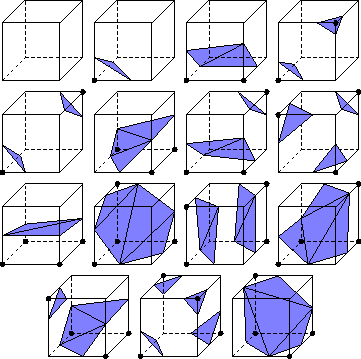
\includegraphics[scale=0.7]{mcCases.png}
  \caption{\label{mcCases} 15 possible cases in the marching cubes algorithm.
}
\end{figure}

The edges start and end points all lie in the middle of the edges of the cube. This allows continuity of the triangulated surface.

Once the triangulation is done, we have to compute and orient the normals for each triangle. The normal can be easily obtain from a simple cross product of two sides of the triangle. The orientation is computed thanks to the isovalue. Considering the barycenter $b$ of $v_1$, $v_2$ and $v_3$ vertices of the triangle, if $value(b + \epsilon n) > isovalue$, then the normal is pointing inward and we must flip it. Else, we do nothing.

%% IMPROVEMENT MC

\newpage
\section*{Conclusion}
\addcontentsline{toc}{section}{Conclusion}

%% CONCLUSION

\newpage
\addcontentsline{toc}{section}{References}
\bibliographystyle{alpha}
\bibliography{biblio}
\end{document}
